\documentclass[border=20mm]{standalone}
\usepackage{bm,amsmath}
\usepackage[RPvoltages]{circuitikz}
\usetikzlibrary{patterns}
\usetikzlibrary{calc}
\begin{document}
    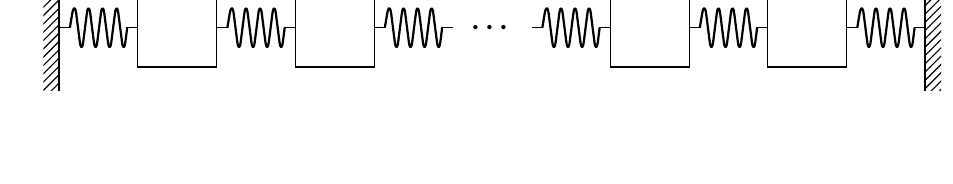
\begin{tikzpicture}
    \begin{circuitikz}    
    \pattern[pattern=north east lines] (-0.2, -0.8) rectangle (0, 0.8);
    \draw[thick] (0, -0.8) -- (0, 0.8);
    \draw (0, 0) to[spring] (1, 0);
    \draw (1, -0.5) rectangle (2, 0.5);
    \draw (2, 0) to[spring] (3, 0);
    \draw (3, -0.5) rectangle (4, 0.5);
    \draw (4, 0) to[spring] (5, 0);
    \node at (5.5, 0) {$\bm{\cdots}$};    
    \draw (6, 0) to[spring] (7, 0);
    \draw (7, -0.5) rectangle (8, 0.5);
    \draw (8, 0) to[spring] (9, 0);
    \draw (9, -0.5) rectangle (10, 0.5);
    \draw (10, 0) to[spring] (11, 0);
    \pattern[pattern=north east lines] (11, -0.8) rectangle (11.2, 0.8);
    \draw[thick] (11, -0.8) -- (11, 0.8);
    \end{circuitikz}
    \end{tikzpicture}    
\end{document}